%%%%%%%%%%%%%%%%%%%%%%%%%%%%%%%%%%%%%%%%%12pt: grandezza carattere
                                        %a4paper: formato a4
                                        %openright: apre i capitoli a destra
                                        %twoside: serve per fare un
                                        %   documento fronteretro
                                        %report: stile tesi (oppure book)
\documentclass[12pt,a4paper,openright,twoside]{report}
%
%%%%%%%%%%%%%%%%%%%%%%%%%%%%%%%%%%%%%%%%%libreria per scrivere in italiano
\usepackage[italian]{babel}
%
%%%%%%%%%%%%%%%%%%%%%%%%%%%%%%%%%%%%%%%%%libreria per accettare i caratteri
                                        %   digitati da tastiera come � �
                                        %   si pu� usare anche
                                        %   \usepackage[T1]{fontenc}
                                        %   per� con questa libreria
                                        %   il tempo di compilazione
                                        %   aumenta
\usepackage[latin1]{inputenc}
%
%%%%%%%%%%%%%%%%%%%%%%%%%%%%%%%%%%%%%%%%%libreria per impostare il documento
\usepackage{fancyhdr}
%
%%%%%%%%%%%%%%%%%%%%%%%%%%%%%%%%%%%%%%%%%libreria per avere l'indentazione
%%%%%%%%%%%%%%%%%%%%%%%%%%%%%%%%%%%%%%%%%   all'inizio dei capitoli, ...
\usepackage{indentfirst}
%
%%%%%%%%%libreria per mostrare le etichette
%\usepackage{showkeys}
%
%%%%%%%%%%%%%%%%%%%%%%%%%%%%%%%%%%%%%%%%%libreria per inserire grafici
\usepackage{graphicx}
%
%%%%%%%%%%%%%%%%%%%%%%%%%%%%%%%%%%%%%%%%%libreria per utilizzare font
                                        %   particolari ad esempio
                                        %   \textsc{}
\usepackage{newlfont}
%
%%%%%%%%%%%%%%%%%%%%%%%%%%%%%%%%%%%%%%%%%librerie matematiche
\usepackage{amssymb}
\usepackage{amsmath}
\usepackage{latexsym}
\usepackage{amsthm}
\usepackage{alltt, fancyvrb, url}
\usepackage{graphicx}
\usepackage{subfigure}
\usepackage{wrapfig}
\usepackage{float}
\usepackage{enumitem}
\usepackage{amsmath}
\graphicspath{ {Report/img/} }
%
\oddsidemargin=30pt \evensidemargin=20pt%impostano i margini
\hyphenation{sil-la-ba-zio-ne pa-ren-te-si}%serve per la sillabazione: tra parentesi 
					   %vanno inserite come nell'esempio le parole 
%					   %che latex non riesce a tagliare nel modo giusto andando a capo.

%
%%%%%%%%%%%%%%%%%%%%%%%%%%%%%%%%%%%%%%%%%comandi per l'impostazione
                                        %   della pagina, vedi il manuale
                                        %   della libreria fancyhdr
                                        %   per ulteriori delucidazioni
\pagestyle{fancy}\addtolength{\headwidth}{20pt}
\renewcommand{\chaptermark}[1]{\markboth{\thechapter.\ #1}{}}
\renewcommand{\sectionmark}[1]{\markright{\thesection \ #1}{}}
\rhead[\fancyplain{}{\bfseries\leftmark}]{\fancyplain{}{\bfseries\thepage}}
\cfoot{}
%%%%%%%%%%%%%%%%%%%%%%%%%%%%%%%%%%%%%%%%%
\linespread{1.3}                        %comando per impostare l'interlinea
%%%%%%%%%%%%%%%%%%%%%%%%%%%%%%%%%%%%%%%%%definisce nuovi comandi
%

\begin{document}
	
	\begin{abstract}
		Questa tesi si pone l'obbiettivo di affrontare ed analizzare un problema di \textit{pathfinding} partendo da uno studio su di alcuni algoritmi per la ricerca del percorso pi� breve su classici grafi, per poi, dopo alcune ottimizzazioni, lavorare con grafi che utilizzano due pesi per ogni arco, considerando l'insieme di soluzioni pi� soddisfacenti.
		
		Dato che, lo studio di algoritmi per la ricerca dei percorsi pi� brevi nei grafi � piuttosto celebre in letteratura, � ormai facile elaborare un'implementazione che permetta di risolvere questo problema, verr� effettuata quindi una rapida implementazione ed analisi. Differente � il discorso per agli algoritmi che lavorano in grafi con pi� pesi, per i quali � pi� difficile reperire implementazioni ed analisi. Inoltre, essendo un lavoro di ottimizzazione mi concentrer� sull'analisi di grafi con due pesi, seppur alcuni algoritmi siano applicabili anche a grafi con un pi� vasta moltitudine di valori.
		%
		
	\end{abstract}
	
\begin{titlepage}                       %crea un ambiente libero da vincoli 
                                        %   di margini e grandezza caratteri:
                                        %   si pu\`o modificare quello che si
                                        %   vuole, tanto fuori da questo
                                        %   ambiente tutto viene ristabilito
%
\thispagestyle{empty}                   %elimina il numero della pagina
\topmargin=6.5cm                        %imposta il margina superiore a 6.5cm
\raggedleft                             %incolonna la scrittura a destra
\large                                  %aumenta la grandezza del carattere
                                        %   a 14pt
\em                                     %emfatizza (corsivo) il carattere
Dedico questo mio modesto lavoro a tutti coloro\\
Che mi sono stati vicini e mi hanno sostenuto\\
In questa piccola parte di un ancora lungo e faticoso cammino\\
In particolare alla mia famiglia \ldots                      %\ldots lascia tre puntini
\newpage                                %va in una pagina nuova
%
%%%%%%%%%%%%%%%%%%%%%%%%%%%%%%%%%%%%%%%%
\clearpage{\pagestyle{empty}\cleardoublepage}%non numera l'ultima pagina sinistra
\end{titlepage}


%\chapter*{Introduzione}                 %crea l'introduzione (un capitolo
                                        %   non numerato)
%%%%%%%%%%%%%%%%%%%%%%%%%%%%%%%%%%%%%%%%%imposta l'intestazione di pagina
%\rhead[\fancyplain{}{\bfseries
%INTRODUZIONE}]{\fancyplain{}{\bfseries\thepage}}
%\lhead[\fancyplain{}{\bfseries\thepage}]{\fancyplain{}{\bfseries
%INTRODUZIONE}}
%%%%%%%%%%%%%%%%%%%%%%%%%%%%%%%%%%%%%%%%%aggiunge la voce Introduzione
                                        %   nell'indice
%\addcontentsline{toc}{chapter}{Introduzione}
%Questa \`e l'introduzione.
%%%%%%%%%%%%%%%%%%%%%%%%%%%%%%%%%%%%%%%%%non numera l'ultima pagina sinistra
%\clearpage{\pagestyle{empty}\cleardoublepage}
\tableofcontents                        %crea l'indice
%%%%%%%%%%%%%%%%%%%%%%%%%%%%%%%%%%%%%%%%%imposta l'intestazione di pagina
\rhead[\fancyplain{}{\bfseries\leftmark}]{\fancyplain{}{\bfseries\thepage}}
\lhead[\fancyplain{}{\bfseries\thepage}]{\fancyplain{}{\bfseries
INDICE}}
%%%%%%%%%%%%%%%%%%%%%%%%%%%%%%%%%%%%%%%%%non numera l'ultima pagina sinistra
\clearpage{\pagestyle{empty}\cleardoublepage}
\listoffigures                          %crea l'elenco delle figure
%%%%%%%%%%%%%%%%%%%%%%%%%%%%%%%%%%%%%%%%%non numera l'ultima pagina sinistra
\clearpage{\pagestyle{empty}\cleardoublepage}
\listoftables                           %crea l'elenco delle tabelle
%%%%%%%%%%%%%%%%%%%%%%%%%%%%%%%%%%%%%%%%%non numera l'ultima pagina sinistra
\clearpage{\pagestyle{empty}\cleardoublepage}

\chapter{Introduzione}                %crea il capitolo
%%%%%%%%%%%%%%%%%%%%%%%%%%%%%%%%%%%%%%%%%imposta l'intestazione di pagina
\lhead[\fancyplain{}{\bfseries\thepage}]{\fancyplain{}{\bfseries\rightmark}}
\pagenumbering{arabic}                  %mette i numeri arabi
L'algoritmo di Dijkstra � largamente utilizzato in ambiti dove i problemi di routing riguardano grafi dove sono presenti valori statici non negativi. Questo celebre algoritmo per� prende in considerazione una sola ``dimensione" dei costi;  se, ad esempio, ci fosse la necessit� di calcolare il percorso in un grafo da un nodo \textit{sorgete} ad uno  \textit{destinazione} questo troverebbe il percorso addizionando volta per volta il peso relativo all'arco che connette due nodi che vengono "visitati" dall'algoritmo. Ma il problema si ha appunto nel momento in cui si hanno due o pi� criteri che relazionano due nodi; ad esempio la distanza e il pericolo. In questo caso si potrebbe scegliere tra diversi percorsi (seppur rappresentati all'interno di un grafo), ma non per forza il pi� corto � anche il pi� sicuro o vice versa. La ricerca di un percorso breve in termini di differenti criteri (molto pi� semplicemente in inglese `\textit{Muticriteria Shortest Paths Problem}') ha lo scopo di ottimizzare i costi dal nodo sorgente a quello di destinazione.\\
In generale non c'� una sola soluzione ottimale, bens� un insieme di possibili soluzioni, anche dette soluzioni ``non dominate" (verr� in seguito approfondito il significato di questa espressione). L'obiettivo di questo progetto � dunque quello di implementare l'algoritmo migliore che possa trovare questo insieme di soluzioni non solo minimizzando il primo o il secondo peso, ma la loro relazione.

\vspace{5mm}

\begin{figure}[H]
	\centering
	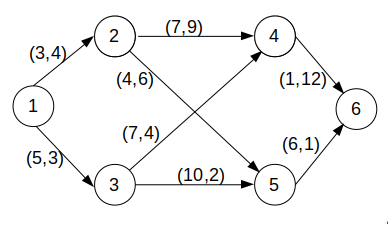
\includegraphics[width=\linewidth]{exampleGraph1}
	\caption{Grafo d'esempio.}
	\label{fig:graphExample}
\end{figure}

\begin{table}[h]
	\centering
	\begin{tabular}{|c|c|c|}
		\hline
		$p1$ & $1\to2\to4\to6$ & (11, 25) \\ \hline
		$p2$ & $1\to2\to5\to6$ & (13, 11)  \\ \hline
		$p3$ & $1\to3\to5\to6$ & (21, 6)  \\ \hline
		$p4$ & $1\to3\to4\to6$ & (13, 18)  \\ \hline
	\end{tabular}
	\caption{Soluzione del grafo}
	\label{tab:graphExample}
\end{table}

La fig.\ref{fig:graphExample} mostra un esempio di grafo a due criteri. Ogni nodo � numerato $\{1,2,\dots,6\}$ ed i pesi presenti sugli archi sono rappresentati come una coppia di valori $(a,b)$. Se considerassimo il primo peso la distanza e il secondo peso, ad esempio, il pericolo, avremo i percorsi $p1$ e $p3$ come il pi� corto ed il pi� sicuro rispettivamente, differentemente $p2$ � una soluzione definita ``non dominata", infatti comprende un percorso pi� lungo rispetto a $p1$, ma al contempo pi� sicuro, mentre percorre un cammino pi� pericoloss, ma pi� corto rispetto a ``p3". $p4$ infine segue un percorso che non risulta vantaggioso ne per il primo valore ne per il secondo, in quanto non porta nessun vantaggio rispetto a $p2$ (la definizione formale di ``soluzione dominata" sar� formulata nel cap.3).
\section{Formulazione Matematica}                 %crea la sezione
Sia definita $G(N,A)$ un grafo orientato composto da un insieme finito di nodi (o vertici) $N = \{0,1,\dots,n\}$ e $A \subseteq N\times N $ di archi direzionati. Ogni arco pu� essere rappresentato come una coppia ordinata $(i,j)$, dove $i\in N$, $j \in N$ ed entrambi due nodi differenti ($i\neq j$) in $G(N,A)$.\\
Sia dunque definito $c^k_{i,j}$ dove $(i,j)\in A$ e $1\leq k \leq 2$ (dato che si tratta di un grafo con due pesi ad ogni arco) che rappresentano i costi relativi ad ogni arco. Considerando quindi due nodi del grafo, chiamati $s$ e $t$, dove $s,t\in N$, i quali rappresentano rispettivamente il nodo da cui iniziano i percorsi che cerchiamo (\textit{source}) ed il nodo terminale (\textit{target}).
            
%dei quali noi vogliamo trovare uno o pi� percorsi
Un cammino $p_{s,t}$ pu� essere rappresentato come una sequenza di nodi e archi, avente la seguente forma: $p_{s,t} = \{s, (s, i_1), i_1, \dots, i_{l}, (i_l,t), t\}$.\\
\'E dunque possibile affermare che ogni $c^k_{i,j}$ rappresenta il costo di uno dei $k$ pesi di ogni arco $(i,j)$, quindi il costo totale dell'intero cammino � rappresentato nel modo seguente:\\

\begin{gather}(c^1(p_{s,t}), c^2(p_{s,t}))\end{gather}
\begin{gather}c^1(p_{s,t})=\sum_{(i,j)\in p}c^1_{i,j}\end{gather}
\begin{gather}c^2(p_{s,t})=\sum_{(i,j)\in p}c^2_{i,j}\end{gather}
Il nostro scopo � quello di \textbf{minimizzare} la ($1.2$) o la ($1.3$) e dunque ottenere lo ``spettro" di soluzioni che  � presente tra le due. Ad esempio considerando il caso succitato dove il primo peso rappresenta la lunghezza ed il secondo il pericolo, minimizzando la ($1.2$) otterremmo il percorso pi� breve, altrimenti il pi� sicuro.

\begin{verbatim}
include stocazzo.h
\end{verbatim}


\section{Seconda Sezione}
Ora vediamo un elenco puntato:
\begin{itemize}                         %crea un elenco puntato
\item primo oggetto
\item secondo oggetto
\end{itemize}

\section{Altra Sezione}
Vediamo un elenco descrittivo:
\begin{description}                     %crea un elenco descrittivo
  \item[OGGETTO1] prima descrizione;
  \item[OGGETTO2] seconda descrizione;
  \item[OGGETTO3] terza descrizione.
\end{description}
%%%%%%%%%%%%%%%%%%%%%%%%%%%%%%%%%%%%%%%%%crea una sottosezione
\subsection{Altra SottoSezione}
%%%%%%%%%%%%%%%%%%%%%%%%%%%%%%%%%%%%%%%%%crea una sottosottosezione
\subsubsection{SottoSottoSezione}Questa sottosottosezione non viene
numerata, ma \`e solo scritta in grassetto.
\section{Altra Sezione}                 %crea una sottosezione
Vediamo la creazione di una tabella; la tabella \ref{tab:uno}
(richiamo il nome della tabella utilizzando la label che ho messo sotto):
la facciamo di tre righe e tre colonne, la prima colonna
``incolonnata'' a destra (r) e le altre centrate (c):\\
\begin{table}[h]                        %ambiente tabella
                                        %(serve per avere la legenda)
\begin{center}                          %centra nella pagina la tabella
\begin{tabular}{r|c|c}                  %tre colonne con righe verticali
                                        %   prodotte con |
\hline \hline                           %inserisce due righe orizzontali
$(1,1)$ & $(1,2)$ & $(1,3)$\\           %& separa le colonne e con
\hline                                  %inserisce una riga orizzontale
$(2,1)$ & $(2,2)$ & $(2,3)$\\           %  \\ va a capo
\hline                                  %inserisce una riga orizzontale
$(3,1)$ & $(3,2)$ & $(3,3)$\\
\hline \hline                           %inserisce due righe orizzontali
\end{tabular}
\caption[legenda elenco tabelle]{legenda tabella}\label{tab:uno}
\end{center}
\end{table}
\section{Altra Sezione}\label{sec:prova}%posso mettere le label anche
                                        %   alle section
\subsection{Listati dei programmi}
\subsubsection{Primo Listato}
\begin{verbatim}
        In questo ambiente     posso scrivere      come voglio,
lasciare gli spazi che voglio e non % commentare quando voglio
e ci sar� scritto tutto.
Quando lo uso � meglio che disattivi il Wrap del WinEdt
\end{verbatim}
%%%%%%%%%%%%%%%%%%%%%%%%%%%%%%%%%%%%%%%%%non numera l'ultima pagina sinistra
\clearpage{\pagestyle{empty}\cleardoublepage}
%%%%%%%%%%%%%%%%%%%%%%%%%%%%%%%%%%%%%%%%%per fare le conclusioni
\chapter*{Conclusioni}
%%%%%%%%%%%%%%%%%%%%%%%%%%%%%%%%%%%%%%%%%imposta l'intestazione di pagina
\rhead[\fancyplain{}{\bfseries
CONCLUSIONI}]{\fancyplain{}{\bfseries\thepage}}
\lhead[\fancyplain{}{\bfseries\thepage}]{\fancyplain{}{\bfseries
CONCLUSIONI}}
%%%%%%%%%%%%%%%%%%%%%%%%%%%%%%%%%%%%%%%%%aggiunge la voce Conclusioni
                                        %   nell'indice
\addcontentsline{toc}{chapter}{Conclusioni} Queste sono le
conclusioni.\\
In queste conclusioni voglio fare un riferimento alla
bibliografia: questo \`e il mio riferimento \cite{K3,K4}.
%%%%%%%%%%%%%%%%%%%%%%%%%%%%%%%%%%%%%%%%%imposta l'intestazione di pagina
\renewcommand{\chaptermark}[1]{\markright{\thechapter \ #1}{}}
\lhead[\fancyplain{}{\bfseries\thepage}]{\fancyplain{}{\bfseries\rightmark}}
\appendix                               %imposta le appendici
\chapter{Prima Appendice}               %crea l'appendice
In questa Appendice non si \`e utilizzato il comando:\\
%%%%%%%%%%%%%%%%%%%%%%%%%%%%%%%%%%%%%%%%%\verb"" � equivalente all'
                                        %   ambiente verbatim,
                                        %   ma si utilizza all'interno
                                        %   di un discorso.
\verb"\clearpage{\pagestyle{empty}\cleardoublepage}", ed infatti
l'ultima pagina 8 ha l'intestazione con il numero di pagina in
alto.
%%%%%%%%%%%%%%%%%%%%%%%%%%%%%%%%%%%%%%%%%imposta l'intestazione di pagina
\rhead[\fancyplain{}{\bfseries \thechapter \:Prima Appendice}]
{\fancyplain{}{\bfseries\thepage}}
\chapter{Seconda Appendice}             %crea l'appendice
%%%%%%%%%%%%%%%%%%%%%%%%%%%%%%%%%%%%%%%%%imposta l'intestazione di pagina
\rhead[\fancyplain{}{\bfseries \thechapter \:Seconda Appendice}]
{\fancyplain{}{\bfseries\thepage}}
\begin{thebibliography}{90}             %crea l'ambiente bibliografia
\rhead[\fancyplain{}{\bfseries \leftmark}]{\fancyplain{}{\bfseries
\thepage}}
%%%%%%%%%%%%%%%%%%%%%%%%%%%%%%%%%%%%%%%%%aggiunge la voce Bibliografia
                                        %   nell'indice
\addcontentsline{toc}{chapter}{Bibliografia}
%%%%%%%%%%%%%%%%%%%%%%%%%%%%%%%%%%%%%%%%%provare anche questo comando:
%%%%%%%%%%%\addcontentsline{toc}{chapter}{\numberline{}{Bibliografia}}
\bibitem{K1} Primo oggetto bibliografia.
\bibitem{K2} Secondo oggetto bibliografia.
\bibitem{K3} Terzo oggetto bibliografia.
\bibitem{K4} Quarto oggetto bibliografia.
\end{thebibliography}
%%%%%%%%%%%%%%%%%%%%%%%%%%%%%%%%%%%%%%%%%non numera l'ultima pagina sinistra
\clearpage{\pagestyle{empty}\cleardoublepage}
\chapter*{Ringraziamenti}
\thispagestyle{empty}
Qui possiamo ringraziare il mondo intero!!!!!!!!!!\\
Ovviamente solo se uno vuole, non \`e obbligatorio.
\end{document}
